\documentclass[12pt]{article}

% Set the page to be letter paper and have small margins
\usepackage{geometry}
\geometry{letterpaper, left=15mm, right=15mm, top=15mm, bottom=20mm}

% LuaLaTeX font setup
\usepackage{fontspec}
\usepackage{unicode-math}

% Text font
\setmainfont{DejaVu Serif}

% Math font
\setmathfont{STIX Two Math}

\allowdisplaybreaks[1]

\usepackage{standalone}
\usepackage{parskip}
\usepackage{amsmath}
\usepackage{amsthm}
\usepackage{multicol}
\usepackage{graphicx}
\usepackage{pgfplots}
\pgfplotsset{compat=1.18}
\usepackage{cancel}
\usepackage{xcolor}
\usepackage[utf8]{inputenc}
\usepackage{float}
\usepackage{graphicx}
\usepackage{pdfpages}
\usepackage{booktabs}

% \usepackage{hyperref}
\usepackage{cleveref}


\usepackage{titlesec}
\titleformat{\section}{\normalfont\normalsize\bfseries}{\thesection.}{1em}{}
\titleformat{\subsection}{\normalfont\normalsize\bfseries\itshape}{\thesubsection}{1em}{}

\usepackage{enumitem}
\setlist[enumerate, 1]{label=\textbf{\arabic*}.}
\setlist[enumerate, 2]{label=\textbf{\alph*}.}

% \usepackage[style=ieee]{biblatex}
% \addbibresource{src/refs.bib}

\makeatletter
\newcommand{\course}[1]{\def\@course{#1}}

\renewcommand{\maketitle}{
    \noindent
    \@author \hfill \@course \newline
    \@date
    \begin{center}
        \large\textbf{\@title}
    \end{center}
    \bigskip
}

\author{Jeffrey Morris}
\course{MATH 4306-010}
\date{\today}


\begin{document}
\begin{align*}
    a_0= & \frac{1}{2\pi}\int_{-\pi}^{\pi}f(x)\,dx           \\
    a_0= & \frac{1}{\pi}\int_{0}^{\pi}f(x)\,dx               \\
    a_0= & \frac{1}{\pi}\int_{0}^{\pi}x\,dx                  \\
    a_0= & \frac{1}{\pi}\left[\frac{x^2}{2}\right]_{0}^{\pi} \\
    a_0= & \frac{1}{\pi}\cdot\frac{\pi^2}{2}                 \\
    a_0= & \boxed{\frac{\pi}{2}}
\end{align*}
\begin{align*}
    a_n= & \frac{1}{\pi}\int_{-\pi}^{\pi}f(x)\cos(nx)\,dx                                                                            \\
    a_n= & \frac{2}{\pi}\int_{0}^{\pi}f(x)\cos(nx)\,dx                                                                               \\
    a_n= & \frac{2}{\pi}\int_{0}^{\pi}x\cos(nx)\,dx                                                                                  \\
    a_n= & \frac{2}{\pi}\left[\left.\frac{x\sin(nx)}{n}\right|_{0}^{\pi}-\int_{0}^{\pi}\frac{\sin(nx)}{n}\,dx\right]                 \\
    a_n= & \frac{2}{\pi}\left[\left(\frac{\pi\cancelto{0}{\sin(nx)}}{n}-0\right)-\left.\frac{-\cos(nx)}{n^2}\right|_{0}^{\pi}\right] \\
    a_n= & \frac{2}{\pi}\left(\frac{\cos(n\pi)}{n^2}-\frac{\cancelto{1}{\cos(0)}}{n^2}\right)                                        \\
    a_n= & \frac{2}{\pi}\left(\frac{(-1)^n}{n^2}-\frac{1}{n^2}\right)                                                                \\
    a_n= &
    \boxed{
        \begin{cases}
            0,                 & \text{if } n \text{ is even} \\
            \frac{-4}{n^2\pi}, & \text{if } n \text{ is odd}
        \end{cases}
    }
\end{align*}
\newpage
\begin{gather*}
    b_n=\frac{1}{\pi}\int_{-\pi}^{\pi}f(x)\sin(nx)\,dx \\
    \text{Because $f(x)$ is odd, $b_n=\boxed{0}$}
\end{gather*}
\begin{center}
    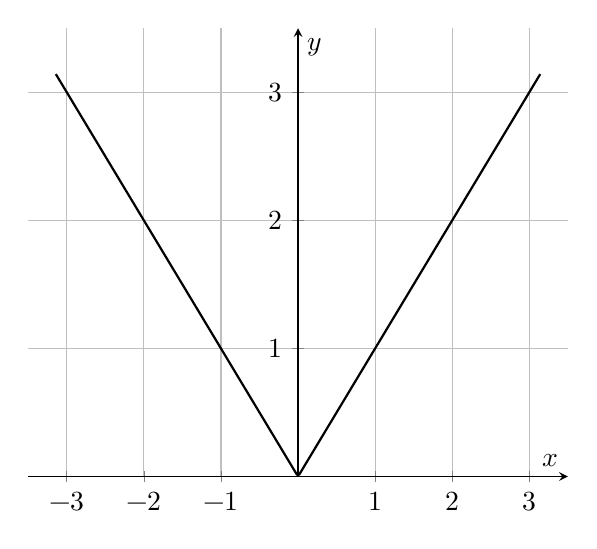
\begin{tikzpicture}
        \begin{axis}[
                axis lines=middle,
                grid=both,
                xmin=-3.5, xmax=3.5,
                ymin=0, ymax=3.5,
                xlabel={$x$}, ylabel={$y$},
                samples=200,
                domain=-pi:pi,
            ]
            \addplot[thick]{abs(x)};
        \end{axis}
    \end{tikzpicture}
\end{center}
\end{document}